\documentclass[a4paper,12pt]{article}
\usepackage{amsmath}
\usepackage{amssymb}
\usepackage[polish]{babel}
\usepackage{polski}
\usepackage[utf8]{inputenc}
\usepackage{indentfirst}
\usepackage{geometry}
\usepackage{array}
\usepackage[pdftex]{color,graphicx}
\usepackage{subfigure}
\usepackage{afterpage}
\usepackage{setspace}
\usepackage{color}
\usepackage{wrapfig}
\usepackage{listings}
\usepackage{datetime}
\renewcommand{\onehalfspacing}{\setstretch{1.6}}
\geometry{tmargin=2.5cm,bmargin=2.5cm,lmargin=2.5cm,rmargin=2.5cm}
\setlength{\parindent}{1cm}
\setlength{\parskip}{0mm}
\newenvironment{lista}{
\begin{itemize}
  \setlength{\itemsep}{1pt}
  \setlength{\parskip}{0pt}
  \setlength{\parsep}{0pt}
}{\end{itemize}}
\newcommand{\linia}{\rule{\linewidth}{0.4mm}}
\definecolor{lbcolor}{rgb}{0.95,0.95,0.95}
\lstset{
    backgroundcolor=\color{lbcolor},
    tabsize=4,
  language=C++,
  captionpos=b,
  tabsize=3,
  frame=lines,
  numbers=left,
  numberstyle=\tiny,
  numbersep=5pt,
  breaklines=true,
  showstringspaces=false,
  basicstyle=\footnotesize,
  identifierstyle=\color{magenta},
  keywordstyle=\color[rgb]{0,0,1},
  commentstyle=\color{Darkgreen},
  stringstyle=\color{red}
  }
\begin{document}
\noindent
\begin{tabular}{|c|p{11cm}|c|} \hline 
Grupa Wtorek 9.15 & Michał Jaworek Marcin Kaciuba & \ddmmyyyydate\today \tabularnewline
\hline 
\end{tabular}


\section*{Algorytm Smitha-Watermana - poszukiwanie optymalnych lokalnych dopasowań sekwencji }

\section*{Algorytm Smitha-Watermana }
Algorytm bazujący na programowaniu dynamicznym umożliwiający poszukiwanie optymalnych lokalnych dopasowań sekwencji.
Jest często wykorzystywany w bioinformatyce do poszukiwań dopasowań sekwencji nukleotydów i aminokwasów.

\begin{figure}[h]
  \vspace{5pt}
  \centering
  \begin{center}
  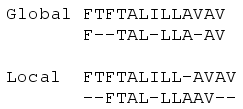
\includegraphics[width=0.65\textwidth]{documentation/images/global-local-alignment.png}
  \end{center}
  \caption{Dopasowanie lokalne a globalne}
 \end{figure}
Trochę o samym algorytmie... 

\section*{Implementacja algorytmu na GPU}
...

\section*{Przeprowadzone testy}

\section*{Wnioski}






\end{document}
